% !TEX root =  free221.tex
\chapter{The Integral}
In this chapter we define the integral of a function on an interval $[a,b]$,
introduce the Fundamental Theorem of Calculus relating integration and
differentiation, and develop basic techniques for computing integrals.

The most common interpretation of the integral is in terms of the area under the
graph of the given function, so that is where we begin.


\section{Area under a Graph} %{{{1
Let $f$ be a function which is defined on an interval $a\leq x\leq
b$ and assume it is positive (so that its graph lies above
the $x$ axis). \textit{How large is the area of the region caught
  between the $x$ axis, the graph of $y=f(x)$ and the vertical lines
  $y=a$ and $y=b$?}
\begin{figure}[h]
    \parbox{0.45\textwidth}{
    \begin{picture} (150.000000,70.307692)(0,0)
    \put(0.0, 0.0){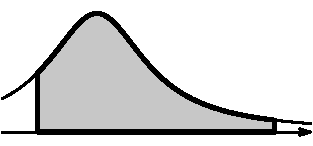
\includegraphics{08AreaUnderGraph.pdf}}
        \put( 16.08,  -5.31){\sffamily\itshape $a$}
    \put(129.92,  -5.31){\sffamily\itshape $b$}
    \put( 78.00,  38.15){\sffamily\itshape $y=f(x)$}
\end{picture}
}
    \parbox{0.45\textwidth}{
    \begin{picture} (150.000000,70.307692)(0,0)
    \put(0.0, 0.0){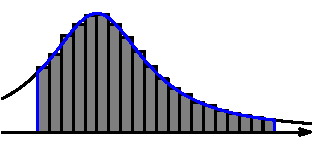
\includegraphics{08Riemann-fine.pdf}}
        \put( 17.08,  -7.31){\sffamily\itshape $a$}
    \put(129.92,  -7.31){\sffamily\itshape $b$}
\end{picture}
}
\end{figure}
We can try to compute this area (on the left here) by approximating
the region with many thin rectangles (on the right).  The idea is that
even though we don't know how to compute the area of a region bounded
by arbitrary curves, we do know how to find the area of one or more
rectangles.

To write formulas for the area of those rectangles we first have to
introduce some notation -- have a look at Figure~\ref{fig:08Riemann}
before reading on.  To make the approximating region, we choose a
\emph{partition} of the interval $[a, b]$: we pick numbers
$x_1<\cdots<x_n$ with
\[
a=x_0 < x_1 < x_2 < \cdots < x_{n-1}< x_n = b.
\]
These numbers split the interval $[a, b]$ into $n$ sub-intervals
\[
[x_0, x_1], \quad [x_1, x_2],\quad \ldots,\quad [x_{n-1}, x_n]
\]
whose lengths are
\[
\Delta x_1 = x_1-x_0, \quad \Delta x_2 = x_2 - x_1, \quad\ldots, \quad
\Delta x_n = x_n-x_{n-1}.
\]
In each interval $[x_{k-1},x_k]$, we choose a \emph{sample point} $c_k$: thus in
the first interval we choose some number $c_1$ such that $x_0\leq c_1\leq x_1$,
in the second interval we choose some $c_2$ with $x_1\leq c_2\leq x_2$, and so
forth. (See Figure~\ref{fig:08Riemann}.)

We then define $n$ rectangles: the base of the $k^{\textrm{th}}$ rectangle is
the interval $[x_{k-1}, x_k]$ on the $x$-axis, while its height is $f(c_k)$
(here $k$ can be any integer from 1 to $n$).

The area of the $k^{\textrm{th}}$ rectangle is the product of its
height and width, which is $f(c_k)\Delta x_k$.  Adding up all the rectangles'
areas yields
\begin{equation}\label{eq:09riemann-sum}
  R = f(c_1)\Delta x_1 + f(c_2) \Delta x_2 + \cdots + f(c_n)\Delta x_n.
\end{equation}
This kind of sum is called a \emph{Riemann sum.}
\begin{figure}[t]
  \centering
  
    \begin{picture} (300.000000,185.384615)(0,0)
    \put(0.0, 0.0){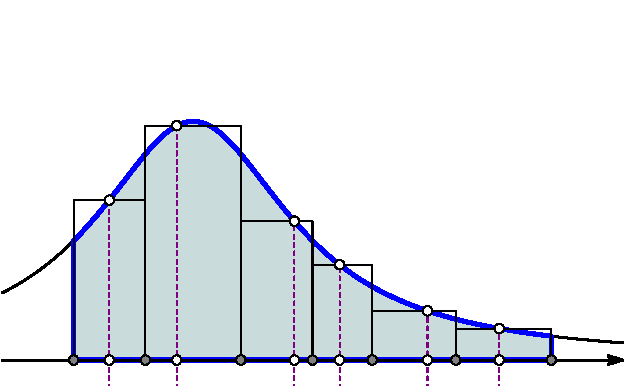
\includegraphics{08Riemann.pdf}}
        \put( 35.38,   0.46){\sffamily\itshape \makebox[0pt][r]{$a=x_0$}}
    \put( 52.45, -11.54){\sffamily\itshape \makebox[0pt][c]{$c_1$}}
    \put( 69.77,   0.46){\sffamily\itshape \makebox[0pt][c]{$x_1$}}
    \put( 84.82, -11.54){\sffamily\itshape \makebox[0pt][c]{$c_2$}}
    \put(115.62,   0.46){\sffamily\itshape \makebox[0pt][c]{$x_2$}}
    \put(141.32, -11.54){\sffamily\itshape \makebox[0pt][c]{$c_3$}}
    \put(150.00,   0.46){\sffamily\itshape \makebox[0pt][c]{$x_3$}}
    \put(162.98, -11.54){\sffamily\itshape \makebox[0pt][c]{$c_4$}}
    \put(178.65,   0.46){\sffamily\itshape \makebox[0pt][c]{$x_4$}}
    \put(205.20, -11.54){\sffamily\itshape \makebox[0pt][c]{$c_5$}}
    \put(218.77,   0.46){\sffamily\itshape \makebox[0pt][c]{$x_5$}}
    \put(239.65, -11.54){\sffamily\itshape \makebox[0pt][c]{$c_6$}}
    \put(264.62,   0.46){\sffamily\itshape \makebox[0pt][l]{$b=x_6$}}
\end{picture}

  \bigskip
  
  \caption{\textbf{A partition, and a Riemann sum. } Here, the interval
    $a<x<b$ is divided up into six smaller intervals.  In each of
    those intervals a sample point $c_i$ is chosen, and the
    resulting rectangles with heights $f(c_1)$, \ldots\,, $f(c_6)$ are
    drawn.  The total area under the graph of the function is roughly
    equal to the total area of the rectangles.  }
  \label{fig:08Riemann}
\end{figure}

If the rectangles are all sufficiently narrow then we would expect that the total
area of all rectangles should be a good approximation of the area of the region
under the graph.  So we would expect the ``area under the curve'' to be the
limit of Riemann sums like $R$ ``as the partition becomes finer and finer''. A
precise formulation of the definition goes like this:

\begin{definition}
  If $f$ is a function defined on an interval $[a, b]$, then we say
  that
  \[
  \int_a^b f(x) dx = I,
  \]
  read as ``the integral of $f(x)$ from $x=a$ to $b$ equals $I$'', if
  for every $\varepsilon >0$, one can find a $\delta>0$ such that
  \[
  \Bigl|f(c_1)\Delta x_1 + f(c_2) \Delta x_2 + \cdots + f(c_n)\Delta
  x_n -I\Bigr|<\varepsilon
  \]
  holds for every partition all of whose intervals have length $\Delta
  x_k<\delta$ with any arbitrary choice of sample points $c_1$, \dots , $c_n$. 
\end{definition}

This is a perfectly good definition, but it's not even clear that the limit
exists even for comparatively simple functions like $f(x)=x$, let alone for more
complicated functions.  It turns out that, with a fair amount of effort, one can
prove that this limit always exists provided that $f(x)$ is a continuous
function on the interval $[a,b]$.  Even so, it is quite hard to evaluate areas
this way.

\section{When $f$ changes its sign} %{{{1
If the function $f$ is not necessarily positive everywhere in the interval
$a\leq x\leq b$, then we still define the integral in exactly the same way: as a
limit of Riemann sums whose mesh size becomes smaller and smaller.  However the
interpretation of the integral as ``the area of the region between the graph and
the $x$-axis'' has a twist to it.

\begin{figure}[h]
  \centering

  
    \begin{picture} (240.000000,137.081081)(0,0)
    \put(0.0, 0.0){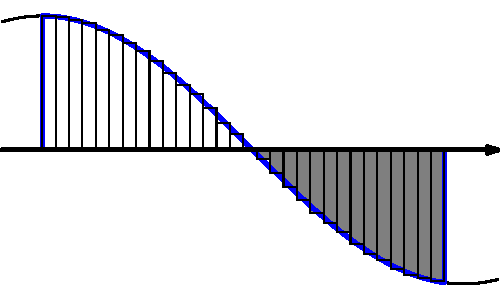
\includegraphics{08Riemann-posandneg.pdf}}
        \put( 19.30,  53.32){\sffamily\itshape $a$}
    \put(211.27,  69.32){\sffamily\itshape $b$}
\end{picture}


  \caption{\textbf{Riemann sum for a function whose sign
    changes.}  Always remember this:\\
    \centerline{\bfseries  INTEGRALS CAN BE NEGATIVE, BUT}
    \centerline{\bfseries AREAS ARE ALWAYS POSITIVE NUMBERS.}\\[2pt]
    The Riemann-sum corresponding to this picture is the total area of
    the rectangles above the $x$-axis \textit{minus} the total area of
    the rectangles below the $x$-axis. }

  \label{fig:08Riemann-posandneg}
\end{figure}

Let $f$ be a function on the interval $a\leq x\leq b$, and form the
Riemann sum
\[
R = f(c_1)\Delta x_1 + f(c_2) \Delta x_2 + \cdots + f(c_n)\Delta x_n
\]
that goes with some partition, and some choice of $c_k$.

When $f$ can be positive or negative, then the terms in the Riemann
sum can also be positive or negative.  If $f(c_k)>0$ then the quantity
$f(c_k)\Delta x_k$ is the area of the corresponding rectangle, but if
$f(c_k)<0$ then $f(c_k)\Delta x_k$ is a negative number, namely
$-1$ times the area of the corresponding rectangle.  The Riemann
sum is therefore the area of the rectangles above the $x$-axis
\textit{minus} the area of the rectangles below the $x$-axis.  Taking
the limit over finer and finer partitions, we conclude that
\[
\int_a^b f(x) dx =
\begin{array}[c]{c}
  \text{area above the $x$-axis, below the graph of $y=f(x)$} \\
  \text{\emph{minus}}\\
  \text{the area below the $x$-axis, above the graph of $y=f(x)$} 
\end{array}
\]

\section{The Fundamental Theorem of Calculus} %{{{1
% !!! Issue: Only half of the fundamental theorem is actually here! The other
% half, about differentiating an integral, is completely missing.
% !!! Issue: There is no discussion whatsoever of the proof of the FToC nor even
% a discussion of why it's intuitively true.
% 
% Sigurd: This should eventually be included.  For now the instructor must present a
% proof in lecture.  The best would be to create an animation that explains the
% whole circle of ideas.
%
\begin{definition}
  A function $F$ is called an \emph{antiderivative} of $f$ on the
  interval $[a, b]$ if one has $F'(x) = f(x)$ for all $x$ with
  $a\leq x \leq b$.
\end{definition}
\smallskip

For instance, $F(x) = \frac12 x^2$ is an antiderivative of $f(x) = x$,
but so are $G(x) = \frac12 x^2+1$ and $H(x) = \frac12x^2 + 2012$.
%  !!! Issue: Needed theorem: Continuous functions have antiderivatives!

\begin{theorem}
  If $f$ is a function whose integral $\int_a^b f(x) dx$ exists, and if
  $F$ is an antiderivative of $f$ on the interval $[a,b]$, then one has
  \begin{equation}
    \label{eq:fundamental-theorem}
    \int_a^b f(x) dx = F(b) - F(a).
  \end{equation}
\end{theorem}
(a proof was given in lecture.)

Because of this theorem the expression on the right appears so often
that various abbreviations have been invented.  We will abbreviate
\[
F(b)-F(a) \stackrel{\text{def}}{=} \bigl. F(x)\bigr]_{x=a}^b =
\bigl.F(x)\bigr]_a^b .
\]

\subsection{Terminology}\label{sec:08terminology} %{{{2
In the integral
\[
\int_a^b f(x)\;dx
\]
the numbers $a$ and $b$ are called the \textit{limits of integration}, the
function $f(x)$ which is being integrated is called \textit{the integrand}, and
the variable $x$ is \textit{integration variable.}

The integration variable is a \textit{dummy variable}.  If we
systematically replace it with another variable, the resulting
integral will still be the same. For instance,
\[
\int_0^1 x^2\,dx = \bigl.\tfrac13 x^3\bigr|_{x=0}^1 = \tfrac13,
\]
and if we replace $x$ by $\varphi$ we still get
\[
\int_0^1 \varphi^2\, d\varphi
= \bigl.\tfrac13 \varphi^3\bigr|_{\varphi=0}^1 = \tfrac13.
\]
Another way to appreciate that the integration variable is a dummy
variable is to look at the Fundamental Theorem again:
\[
\int_a^b f(x)\;dx = F(b) -F(a).
\]
The right hand side tells you that the value of the integral depends
on $a$ and $b$, and has absolutely nothing to do with the variable $x$.

\section{Summation notation} %{{{1
\label{sec:09about-those-dots}
A Riemann sum is a summation with very many terms: more to the point, a Riemann
sum usually has ``$n$ terms'' where $n$ is allowed to vary.  For such a sum we
cannot write all terms in the way we can for a sum that has, say, 25 terms.
This is why our formulas for Riemann sums, such as \eqref{eq:09riemann-sum},
\[
  R = f(c_1)\Delta x_1 + f(c_2) \Delta x_2 + \cdots + f(c_n)\Delta x_n
\]
contain dots ($\cdots$) to represent the terms we didn't explicitly write.
Even though we did not write most of the terms in this sum it is clear what they
are, just from looking at the pattern of the first two and the last term.

If we don't like the ambiguity created by the dots in the Riemann sum, then we
can use summation notation: if we have a sum with $n$ terms, and if we
have a formula $a_k$ for term number $k$ in the sum, then we write
\[
  \sum_{k=1}^n a_k = a_1+a_2+\cdots+a_n.
\]
The expression on the right is pronounced as ``the sum from $k=1$ to $n$ of
$a_k$''.  For example,
\[
  \sum_{k=3}^7 k^2 = 3^2 + 4^2 + 5^2 + 6^2 + 7^2,
\]
which adds up to $9+16+25+36+49 = 135$.

With this notation we can write the Riemann sum \eqref{eq:09riemann-sum} as
\[
  R = f(c_1)\Delta x_1 + f(c_2) \Delta x_2 + \cdots + f(c_n)\Delta x_n
  = \sum_{k=1}^n f(c_k) \Delta x_k.
\]
The advantage of $\Sigma$ notation is that it takes the guesswork out of the
summation:  we don't have to guess what the 23$^{\rm rd}$ term is because there
is a formula in which we can just substitute $k=23$.  If we don't care for the
$\Sigma$ notation (like the author of this text, but perhaps unlike your
instructor) then our writing has to be so clear that the reader can easily
guess what the dots represent when we write them.

Using $\Sigma$ notation our definition of the integral is often written in
the following form
\begin{equation}
  \int_a^b f(x) dx
  =
  \lim_{n\to\infty} \sum_{k=1}^n f(c_k) \Delta x_k.
  \label{eq:09integral-def-using-sigma-notation}
\end{equation}
This way of writing the definition of the integral gives a hint of where the
integral sign came from.  On the right a $\Sigma$ (the greek upper case ``S'')
was used to denote a summation.
\marginpar{\centering\sffamily\itshape\footnotesize%
\framebox{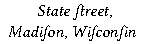
\includegraphics{08long-s.pdf}}\\[1ex]
The ``long s'' from which the integral sign derives.
}
On the left is an integral, which is not really
a sum, but a limit of sums.  To denote it, Leibniz chose an
$S$, which in the typesetting of his time looked like a ``long~s,'' and which today
looks more like an \textit{f} than an \textit{s}.


\section{Problems} %{{{1
\problemfont %{{{3
\begin{multicols}{2}\setlength{\parindent}{0pt}
\problem  %{{{3
\subprob What is a Riemann sum of a function $y=f(x)$ on an interval $a\leq
x \leq b$?

\subprob Compute $\sum_{k=1}^4 \frac{1}{k}$.
\answer %{{{3
$\sum_{k=1}^4 \frac{1}{k}
= \frac{1}{1} +  \frac{1}{2} + \frac{1}{3} + \frac{1}{4}$.

This adds up to $\frac{25}{12}$, but the point of this question was to get the
above answer.
\endanswer

\subprob Compute $\sum_{k=4}^7 2^k$.
\answer %{{{3
$2^4 + 2^5 +2^6 + 2^7$.
\endanswer

\problem Let $f$ be the function $f(x) = 1-x^2$. %{{{3

\subprob Draw the graph of $f(x)$ with $0\le x\le2$.

\subprob Compute the Riemann-sum for the partition
\[
0<\tfrac13<1<\tfrac32<2
\]
of the interval $[a, b] = [0, 2]$ if we choose each $c_k$ to be the
left endpoint of the interval it belongs to.  Draw the corresponding
rectangles (add them to our drawing of the graph of $f$).

\subprob Compute the Riemann-sum you
get if you choose the $c_k$ to be the
right endpoint of the interval it belongs to.  Make a new drawing of
the graph of $f$ and include the rectangles corresponding to the right
endpoint Riemann-sum.
\answer %{{{3
Choosing left endpoints for the $c$'s gives you
\[
f(0)\frac13 + f(\frac13)\frac23 + f(1)\frac12 + f(\frac32)\frac12
=\cdots
\]
Choosing right endpoints gives
\[
f(\frac13)\frac13 + f(1)\frac23 + f(\frac32)\frac12 + f(2)\frac12
\]
\endanswer

\problem \itshape The analog of the Fundamental Theorem for finite sums.\upshape %{{{3
% The wording of this problem needs some work
In this problem you'll compute 
\[
  1+3+5+7+\cdots+159
\]
in a smart way.  First note that there are $80$ terms, and that the $k$th term
is $f(k) = 2k-1$, so you really are going to compute
\[
  f(1) + f(2) + \cdots + f(80).
\]
\subprob Show that for the function $F(k) = k^2$, it is true that $F(k)-F(k-1) =
f(k).$
\answer %{{{3
$F(n) - F(n-1) = n^2 - (n-1)^2 = n^2 - (n^2-2n+1) = 2n-1 = f(n)$.
\endanswer
\subprob Compute $S = f(1)+f(2)+\cdots f(80)$ in terms of the function
$F$.  
\answer %{{{3
Substitute $f(1) = F(1) - F(0)$, $f(2) = F(2) - F(1)$, etc\ldots 

You get many terms, and almost all of them cancel:
\[
\begin{array}{lrcl}
  &f(1) & = & \cancel{F(1)} - F(0) \\
  &f(2) & = & \cancel{F(2)} - \cancel{F(1)} \\
  &f(3) & = & F(3) - \cancel{F(2)} \\
   && \vdots &\\
   &f(79) & = & \cancel{F(79)} - F(78) \\
   +&f(80) & = & F(80) - \cancel{F(79)} \\[4pt]
  \hline      
  &\rule{0pt}{12pt}
  S & = & F(80) - F(0) \\
\end{array}
\]
So the answer is 
\[
  f(1)+\cdots+f(80) = F(80) - F(0).
\]
In the particular example where $f(n)= 2n-1$ you get
\begin{multline*}
  1+3+5+7+\cdots+157+159 \\
  = (80)^2 = 1600.
\end{multline*}
\endanswer

\problem \groupproblem Look at figure \ref{fig:08Riemann} (top). %{{{3
Which choice of intermediate points $c_1$, \ldots, $c_6$ leads to the
smallest Riemann sum?  Which choice would give you the largest
Riemann-sum?

(Note: in this problem you're not allowed to change the division points
$x_i$, only the points $c_i$ in between them.)
\answer %{{{3
The Riemann-sum is the total area of the rectangles, so to get the
smallest Riemann-sum you must make the rectangles as small as
possible.  You can't change their widths, but you can change their
heights by changing the $c_i$.  To get the smallest area we make the
heights as small as possible. So, for the \emph{smallest} possible
Riemann sum choose  $c_i$ to be the point in the interval $[x_i,
x_{i+1}]$ where $f(x)$ attains its minimum.

For the largest possible Riemann sum choose each $c_i$ to be the point
in $[x_i, x_{i+1}]$ where $f(x)$ is maximal.

In this example this means you should choose:  $c_1 = x_1$, $c_2$ somewhere
between $x_1$ and $x_2$ where $f$ has its maximum, $c_3=x_2$, $c_4=x_3$,
$c_5=x_4$, and $c_6 = x_5$.

\endanswer
%
\[
\clubsuit
\]
\begingroup
  \itshape Find an antiderivative $F(x)$ for each of the following
  functions $f(x)$.  Finding antiderivatives involves a fair amount of
  guess work, but with experience it gets easier to guess
  antiderivatives.
\endgroup


\problem $\displaystyle f(x) = 2x+1 $ %{{{3

\problem $\displaystyle f(x) = 1-3x $ %{{{3

\problem $\displaystyle f(x) = x^2-x+11 $ %{{{3

\problem $\displaystyle f(x) = x^4-x^2 $ %{{{3

\problem $\displaystyle f(x) = 1+x+\frac{x^2}{2}+\frac{x^3}{3}+\frac{x^4}{4} $ %{{{3

\problem $\displaystyle f(x) = \frac1x $ %{{{3

\problem $\displaystyle f(x) = e^x $ %{{{3

\problem $\displaystyle f(x) = \frac2x $ %{{{3

\problem $\displaystyle f(x) = e^{2x} $ %{{{3

\problem $\displaystyle f(x) = \frac1{2+x} $ %{{{3

\problem $\displaystyle f(x) = \frac{e^x-e^{-x}}2 $ %{{{3

\problem $\displaystyle f(x) = \frac1{1+x^2} $ %{{{3

\problem $\displaystyle f(x) = \frac{e^x+e^{-x}}2 $ %{{{3

\problem $\displaystyle f(x) = \frac1{\sqrt{1-x^2}} $ %{{{3

\problem $\displaystyle f(x) = \sin x $ %{{{3

\problem $\displaystyle f(x) = \frac2{1-x} $ %{{{3

\problem $\displaystyle f(x) = \cos x $ %{{{3

\problem $\displaystyle f(x) = \cos2x $ %{{{3

\problem $\displaystyle f(x) = \sin(x-\pi/3) $ %{{{3

\problem $\displaystyle f(x) = \sin x + \sin 2x $ %{{{3

\problem $\displaystyle f(x) = 2x(1+x^2)^5$ %{{{3
\[
\heartsuit
\]
\begingroup
  \itshape In each of the following exercises, draw the indicated region and
  compute its area.
\endgroup

\problem The region between the vertical lines $x=0$ and $x=1$, and between the %{{{3
$x$-axis and the graph of $y=x^3$.

\problem The region between the vertical lines $x=0$ and $x=1$, and between the %{{{3
$x$-axis and the graph of $y=x^n$ (here $n>0$, draw for $n=\frac12, 1,
2, 3, 4$).

\problem The region above the graph of $y=\sqrt x$, below the line $y=2$, and %{{{3
between the vertical lines $x=0$, $x=4$.

\problem The bounded region above the $x$-axis and below the graph of $f(x) = x^2-x^3$. %{{{3

\problem The bounded region above the $x$-axis and below the graph of $f(x) = 4x^2-x^4$. %{{{3

\problem The region above the $x$-axis and below the graph of $f(x) = 1-x^4$. %{{{3

\problem The region above the $x$-axis, below the graph of $f(x) = \sin x$, and %{{{3
between $x=0$ and $x=\pi$.

\problem The region above the $x$-axis, below the graph of $f(x) = 1/(1+x^2)$ (a %{{{3
curve known as the \textit{witch of Maria Agnesi}), and between $x=0$ and
$x=1$.

\problem The region between the graph of $y=1/x$ and the $x$-axis, and between %{{{3
$x=a$ and $x=b$ (here $0<a<b$ are constants, e.g.\ choose $a=1$ and $b=
\sqrt2$ if you have something against either letter $a$ or $b$.)

\problem The bounded region below the $x$-axis and above the graph of %{{{3
\[
f(x) = \frac1{1+x} + \frac x2 -1.
\]

\problem Compute %{{{3
\[
\int_0^{1}\sqrt{1-x^2} dx
\]
without finding an antiderivative for $\sqrt{1-x^2}$ (you can find such
an antiderivative, but it's not easy.  This integral is the area of
some region: which region is it, and what is that area?)

\problem \groupproblem Compute these integrals without finding antiderivatives. %{{{3
\[
I = \int_0^{1/2}\sqrt{1-x^2}\,dx
\]
\[
J=\int_{-1}^1 |1-x|\,dx
\]
\[
K=\int_{-1}^1 |2-x|\,dx
\]



\end{multicols}
\noproblemfont

\section{The indefinite integral} %{{{1
\label{sec:indefinite-integral}
The fundamental theorem tells us that in order to compute the integral
of some function $f$ over an interval $[a,b]$ you should first find an
antiderivative $F$ of $f$.  In practice, much of the effort required
to find an integral goes into finding an antiderivative.  In order to
simplify the computation of the integral
\begin{equation}
  \label{eq:08definite-integral}
  \int_a^b f(x) dx = F(b)-F(a)
\end{equation}
the following notation is commonly used for the antiderivative:
\begin{equation}
  \label{eq:08indefinite-integral}
  F(x) = \int f(x) d x .
\end{equation}
For instance,
\[
\int x^2 \;dx = \tfrac13x^3+C,\quad \int \sin 5x\; dx = -\tfrac15\cos 5x+C,
\quad\textrm{etc}\ldots
\]
The integral which appears here does not have the limits of integration
$a$ and $b$.  It is called an \emph{indefinite integral}, as opposed
to the integral in \eqref{eq:08definite-integral} which is called a
\emph{definite integral}.


It is important to distinguish between the two kinds of integrals.
The main differences are listed in
Table~\ref{tbl:def-vs-indef-integrals}.

\begin{table}\sffamily
  \begin{tabular}{@{\extracolsep{2em}}cc}
    \toprule[2pt]
    \bfseries Indefinite integral & \bfseries Definite integral\\[2pt]
    \midrule \\
    $\int f(x) d x$ is a function of $x$.&
    $\int_a^bf(x)d x$ is a number. \\[1ex]
    \begin{minipage}[c]{160pt}
      By definition $\int f(x)d x$ is \textit{any function of $x$
        whose derivative is $f (x)$.}
    \end{minipage} &
    \begin{minipage}[c]{160pt}
      $\int_a^b f(x)d x$ is defined in terms of Riemann sums and can
      be interpreted as the ``area under the graph of $y=f(x)$'' when $f(x)>0$.
    \end{minipage}
    \\[1ex]
    \parbox[t]{160pt}{\vspace{1pt}

      $x$ is not a dummy variable, for example, 
      \ $\int 2xd x=x^2+C$ and $\int 2td t=t^2+C$ are
      functions of different variables, 
      so they are not equal.}&
    \parbox[t]{160pt}{\vspace{1pt}

      $x$ is a dummy variable, for example,  
      $\int_0^1 2xd x=1$, and $\int_0^1 2td t=1$, 
      so $\int_0^1 2xd x=\int_0^1 2td t$.}\\
    \bottomrule[2pt]

  \end{tabular}
  \bigskip
  
  \caption{The differences between \emph{definite} and
  \emph{indefinite} integrals}
  \label{tbl:def-vs-indef-integrals}
\end{table}

\subsection{About ``$+C$''} %{{{2
\label{sec:about-+c}
Let $f (x)$ be a function defined on the interval $[a,b]$.
If $F(x)$ is an antiderivative of $f(x)$ on this interval, then for
any constant $C$ the function $\tilde F(x)=F(x)+C$ will also be an
antiderivative of $f(x)$. So one given function $f(x)$ has many
different antiderivatives, obtained by adding different constants to
one given antiderivative.

\subsection*{Theorem} %{{{2
\itshape
If $F_1 (x)$ and $F_2 (x)$ are antiderivatives of the same function
$f(x)$ on some interval $a\leq x\leq b$, then there is a constant $C$
such that $F_1 (x)=F_2 (x)+C$.\upshape

\begin{proof}
  Consider the difference $G(x)=F_1(x)-F_2(x)$. Then $G'(x) =
  F_1'(x)-F_2'(x)=f(x)-f(x)=0$, so that $G(x)$ must be constant. Hence
  $F_1(x)-F_2(x)=C$ for some constant.
\end{proof}
% !!! Issue: It is not proven or even mentioned anywhere in the differentiation chapters that a function with zero derivative is constant!

It follows that there is some ambiguity in the notation $\int f(x)\, d
x$. Two functions $F_1(x)$ and $F_2(x)$ can both equal $\int f(x)\, d
x$ without equaling each other. When this happens, they ($F_1$ and
$F_2$) differ by a constant. This can sometimes lead to confusing
situations, e.g.\ you can check that
\begin{gather*}
  \int 2\sin x\cos x\, d x = \sin^2 x + C\\
  \int 2\sin x\cos x\, d x = -\cos^2 x + C
\end{gather*}
are both correct. (Just differentiate the two functions $\sin^2x$ and
$-\cos^2x$!) These two answers look different until you realize that
because of the trig identity $\sin^2 x+\cos^2x=1$ they really only
differ by a constant: $\sin^2x= -\cos^2x+1$, and the ``$+1$'' gets absorbed into the $+C$ term.


\begin{center}
  \fbox{\parbox{3in}{\bfseries To avoid this kind of confusion we will
      from now on never forget to include the ``arbitrary constant
      $+C$'' in our answer when we compute an antiderivative.}}
\end{center}


\subsection{You can always check the answer} %{{{2
\label{sec:you-can-always}
Suppose you want to find an antiderivative of a given function $f(x)$
and after a long and messy computation
you get an ``answer'', $F(x)$, but you're not sure if you trust that it's right. Fortunately, it is easy to check: you need only differentiate the $F(x)$ you found, and if $F'(x)$
turns out to be equal to $f(x)$, then your $F(x)$ is indeed an
antiderivative.

For example, suppose that we want to find $\int \ln x\, d x$. My
cousin Louie says it might be $F(x) = x\ln x -x$.  Let's see if he's
right:
\[
\frac{d}{dx}\bigl(x\ln x-x\bigr) = x\cdot\frac1x+1\cdot\ln x-1 = \ln
x.
\]
Who knows how Louie thought of this\footnote{He took math 222 and
  learned to integrate by parts.}, but it doesn't matter: he's right!
We now know that $\int \ln x d x=x\ln x-x+C$.

% !!! TO-DO: rewrite all the entries in this table using operator notation
\begin{table}[hb]
  \centering\sffamily
  \rule[6pt]{\textwidth}{2pt}
  \begin{tabular}{r@{\,$=$\,}lr@{$\,=\,$}lp{36pt}}
      $\displaystyle f(x)$&
    $\displaystyle \frac{dF(x)} {dx} $ &
    $\displaystyle  \int f(x)\, d x  $&
    $\displaystyle  F(x)+C $ &
    \\[3ex]
    \midrule
    $\displaystyle (n+1)x^n $&
    $\displaystyle  \frac{dx^{n+1}} {dx}$ &
    $\displaystyle \int x^{n}\, d x  $&
    $\displaystyle   \frac{x^{n+1}}{n+1}+C$ &
    $n\neq -1$\\[3ex]
    $\displaystyle \frac{1}{x} $&
    $\displaystyle  \frac{d \ln |x|}{dx} $&
    $\displaystyle \int \frac{1}{x}\, d x $&
    $\displaystyle  \ln |x| +C $&
    absolute values!!\\[3ex]
    $\displaystyle e^x $&
    $\displaystyle  \frac{de^x} {dx}$ &
    $\displaystyle \int e^x\, dx $&
    $\displaystyle  e^x +C$& \\[3ex]
    $\displaystyle -\sin x $&
    $\displaystyle  \frac{d \cos x}{dx}$&
    $\displaystyle \int \sin x\, d x  $&
    $\displaystyle   -\cos x+C$\\[3ex]
    $\displaystyle  \cos x  $&
    $\displaystyle  \frac{d  \sin x}{dx}$&
    $\displaystyle \int \cos x\, d x  $&
    $\displaystyle   \sin x+C$\\[3ex]
    $\displaystyle  \tan x  $&
    $\displaystyle  -\frac{d \ln |\cos x|}{dx}$ &
    $\displaystyle \int \tan x $&
    $\displaystyle  -\ln |\cos x|+C$ &
    absolute values!!\\[3ex]
    $\displaystyle  \frac{1}{1+x^{2}} $&
    $\displaystyle   \frac{d \arctan x}{dx}$&
    $\displaystyle \int \frac{1}{1+x^{2}}\, d x  $&
    $\displaystyle   \arctan x+C$\\[3ex]
    $\displaystyle  \frac{1}{\sqrt{1-x^{2}}} $&
    $\displaystyle  \frac{d\arcsin x}{dx} $&
    $\displaystyle \int \frac{1}{\sqrt{1-x^{2}}}\, d x  $&
    $\displaystyle   \arcsin x+C $\\[3ex]
    $\displaystyle  f(x) + g(x) $&
    $\displaystyle  \frac{d F(x) + G(x)} {dx}$&
    $\displaystyle \int \{f(x)+g(x)\} \,dx $&
    $\displaystyle   F(x)+G(x)+C $&
    See \eqref{eq:integral-additive}\\[3ex]
    $\displaystyle  cf(x) $&
    $\displaystyle  \frac{d\, cF(x)} {dx}$&
    $\displaystyle \int cf(x) \,dx $&
    $\displaystyle   cF(x)+C $&
    See \eqref{eq:integral-homogeneous}\\[3ex]
  \end{tabular}
  \smallskip
  \rule[1pt]{\textwidth}{0.3pt}

  To find derivatives and integrals involving $a^x$ instead of $e^x$ use
  $a = e^{\ln a}$,\\
  and thus $a^{x} = e^{x\ln a}$, to rewrite all exponentials as $e^{\ldots}$.
  \smallskip

  The following integral is also useful, but not as important as the
  ones above:
  \[
  \int \frac{ d x}{\cos x} = \frac12 \ln\left(\frac{1+\sin x}{1-\sin x}\right) +C
  \text{ for }\cos x\neq 0.
  \]
  \rule[1pt]{\textwidth}{2pt}
  \caption{The list of the standard integrals everyone should know}
  \label{tbl:standard-integrals}
\end{table}

Table \ref{tbl:standard-integrals} lists a number of antiderivatives which you
should know.  All of these integrals should be familiar from the
differentiation rules we have learned so far, except for the integrals of
$\tan x$ and of $\dfrac1{\cos x}$.  You can check those by differentiation
(using $\ln\frac ab=\ln a-\ln b$ simplifies things a bit).


\section{Properties of the Integral} %{{{1
Just as we had a list of properties for the limits and derivatives of
sums and products of functions, the integral has similar properties.
% except integration by parts does not appear here!

Suppose we have two functions $f(x)$ and $g(x)$ with antiderivatives
$F(x)$ and $G(x)$, respectively.  Then we know that
\[
\frac{d}{dx}\bigl(F(x) + G(x)\bigr) = F'(x) + G'(x) = f(x) + g(x).
\]
In words, $F+G$ is an antiderivative of $f+g$.  Using indefinite
integrals we can write this as
\begin{equation}
  \label{eq:sum-of-antiderivs}
  \int\bigl( f(x) + g(x) \bigr)\, dx =
  \int f(x) \, dx +\int g(x) \, dx.
\end{equation}
Similarly, $\frac{d}{dx}\bigl(cF(x)\bigr) = cF'(x) = cf(x)$ implies
that
\begin{equation}
  \label{eq:constant-times-antideriv}
  \int cf(x) \, dx = c\int f(x) \, dx
\end{equation}
if $c$ is a constant.


These properties imply analogous properties for the definite integral.
For any pair of functions on an interval $[a, b]$ one has
\begin{equation}
  \label{eq:integral-additive}
  \int_a^b\bigl[f(x) + g(x) \bigr] dx = 
  \int_a^b f(x) dx + \int_a^bg(x) dx,
\end{equation}
and for any function $f$ and constant $c$ one has
\begin{equation}
  \label{eq:integral-homogeneous}
  \int_a^b cf(x) dx = c\int_a^bf(x)dx.
\end{equation}

Definite integrals have one other property for which there is no
analog in indefinite integrals: if you split the interval of
integration into two parts, then the integral over the whole is the
sum of the integrals over the parts. The following theorem says it
more precisely.

\subsection{Theorem} %{{{2
\itshape
Given $a<b<c$, and a function on the interval $[a,b]$ then
\begin{equation}
  \label{eq:integral-domain-additive}
  \int_a^b f(x)dx + \int_b^c f(x)dx = \int_a^c f(x)dx .
\end{equation}\upshape%\smallskip


\hangindent180pt\hangafter=3%
\textit{A picture proof, assuming $f(x)>0$. } The drawing shows the
graph of a positive function on some interval $a\leq x\leq c$.  The
region below the graph consists of two pieces, namely the part with
$a\leq x\leq b$ and the part with $b\leq x\leq c$.  The total area
under the graph is the sum of the areas of the two pieces.  Since the
function is positive, the areas are given by the corresponding
integrals.  The total area is\\
\hbox to 180pt{\hspace{60pt}$\displaystyle \int_a^c f(x)dx$.}\\
and it is the sum of the areas of the two smaller regions.  This
implies \eqref{eq:integral-domain-additive}.

\noindent%
\parbox[b][0pt][b]{0.4\textwidth}{\input ../figures/221/08int-atob-plus-int-btoc.pdf_tex }

\textit{A proof using the Fundamental Theorem. } Let $F$ be an
antiderivative of $f$.  Then
\[
\int_a^b f(x)dx = F(b) - F(a) \text{ and } \int_b^c f(x)dx = F(c) -
F(b),
\]
so that
\begin{align*}
   \int_a^b f(x)dx + \int_b^c f(x)dx   &= F(b) - F(a) + F(c) - F(b) \\
  &= F(c) - F(a) \\
  &=\int_a^c f(x)dx.
\end{align*}

\subsection{When the upper integration bound is less than the lower bound} %{{{2
So far we have always assumed that $a<b$ in all indefinite integrals
$\int_a^b \ldots$.  The Fundamental Theorem suggests that when $b<a$,
we should define the integral as
\begin{equation}
  \int_a^bf(x)dx = F(b)-F(a) = -\bigl(F(a)-F(b)\bigr) = -\int_b^a f(x)dx.
\end{equation}
For instance,
\[
\int_1^0 xdx = -\int_0^1 xdx = -\tfrac12.
\]



\section{The definite integral as a function of its integration bounds} %{{{1
\subsection{A function defined by an integral} %{{{2
Consider the expression
\[
I = \int_0^x t^2\, dt.
\]
What does $I$ depend on?  To find out, we calculate the integral
\[
I = \bigl[\tfrac13t^3\bigr]_0^x 
= \tfrac13 x^3 - \tfrac13 0^3
= \tfrac13 x^3.
\]
So the integral depends on $x$.  It does not depend on $t$, since $t$
is a ``dummy variable'' (see \S\ref{sec:08terminology}, where we already
discussed this point).

In this way we can use integrals to define new functions.  For
instance, we could define
\[
I(x) = \int_0^x t^2 dt,
\]
which would be a roundabout way of defining the function $I(x) = x^3/3$.  Again,
since $t$ is a dummy variable we can replace it by any other variable we like.
Thus
\[
I(x) = \int_0^x \alpha^2\, d\alpha
\]
defines the same function (namely, $I(x) = \frac13x^3$).

This example does not really define a new function, in the sense that
we already had a much simpler way of defining the same function,
namely ``$I(x) = x^3/3$.''  An example of a \textit{new} function
defined by an integral is the so called \emph{error function} from
statistics:
\begin{equation}\label{eq:08erf-defined}
  \erf(x) \isdef
  \frac2{\sqrt\pi} \int _0 ^x e^{-t^2}\;dt,
\end{equation}
so that $\erf(x)$ is the area of the shaded region in figure \ref{fig:08erf}.
\begin{figure}[h]
  \centerline{\begin{picture} (270.000000,100.266667)(0,0)
    \put(0.0, 0.0){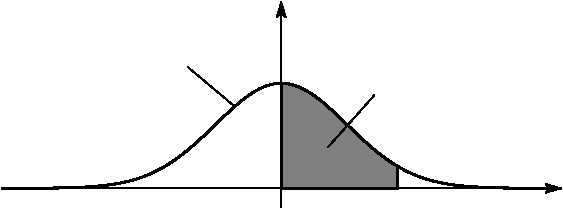
\includegraphics{08erf.pdf}}
        \put(180.67,  55.60){\sffamily\itshape Area $=\erf(x)$}
    \put( 72.33,  75.00){\sffamily\itshape $y=\frac2{\sqrt\pi}e^{-x^2}$}
    \put(190.83,  -2.07){\sffamily\itshape $x$}

\end{picture}
}
  \caption{Definition of the Error function.  The graph is known as
    the ``Bell curve'' or the Gaussian curve.}
  \label{fig:08erf}
\end{figure}
The integral in \eqref{eq:08erf-defined} cannot be computed in terms of the
standard functions (square and higher roots, sine, cosine, exponential and
logarithms).  Since  the integral in \eqref{eq:08erf-defined} occurs very often
in statistics (in relation with the so-called normal distribution) it has been
given its own name, ``$\erf(x)$''.

\subsection{How do you differentiate a function that is defined by an integral?} %{{{2
The answer is simple, for if $f(x) = F'(x)$ then the Fundamental Theorem says
that
\[
\int_a^x f(t) \; dt = F(x) - F(a),
\]
and therefore
\[
\frac d{dx} \int_a^x f(t) \; dt =\frac d{dx}\bigl( F(x) - F(a)\bigr) = F'(x) =
f(x),
\]\marginpar{\sffamily\footnotesize%
  Note that here we use operator notation, as in
  Chapter IV, \S~\ref{sec:04operator-notation}, and that, by definition,\\[2ex]
  \(\displaystyle
  \frac{d} {dx}\int_a^x f(t) dt =\)\\[2ex]
  \null\hfill\(\displaystyle\frac{d \int_a^x f(t) dt} {dx}
  \)}%
i.e.
\[
\frac d{dx} \int_a^x f(t) \; dt = f(x).
\]
A similar calculation gives you
\[
\frac d{dx} \int_x^b f(t) \; dt = -f(x).
\]
So what is the derivative of the error function?
It is
\begin{align*}
  \erf\, '(x) 
  &= \frac d{dx} \left[ \frac2{\sqrt\pi} \int _0 ^x e^{-t^2}\;dt\right] \\
  &= \frac2{\sqrt\pi} \frac d{dx} \left[\int _0 ^x e^{-t^2}\;dt\right] \\
  &=  \frac2{\sqrt\pi} e^{-x^2}.
\end{align*}


\section{Substitution in Integrals} %{{{1
\label{sec:method-substitution}
The Chain Rule says that
\[
\frac{d F(G(x))}{d x } = F'(G(x))\cdot G'(x),
\]
so that
\[
\int F'(G(x))\cdot G'(x) \,d x = F(G(x)) +C.
\]

We can use this result to evaluate new integrals by making substitutions.

\subsection{Example} %{{{2
Consider the function $f(x) = 2x\sin (x^2+3)$. It does not appear in
the list of standard antiderivatives we know by heart. But we do
notice\marginpar{\sffamily\footnotesize%
  With practice it gets easier to recognize what
  substitution could help you compute a specific integral, 
  but even with a lot of practice, substitution is still a matter of trial and error.} that $2x =
\frac{d}{dx} (x^2+3)$. So let's call $G(x)=x^2+3$, and $F(u) = -\cos
u$, then
\[
F(G(x)) = -\cos (x^2+3)
\]
and
\[
\frac{dF(G(x))}{dx} = \underbrace{\sin (x^2+3)}_{F'(G(x))}\cdot
\underbrace{\vphantom{(}2x}_{G'(x)} = f(x),
\]
so that
\begin{equation}
  \label{eq:substitution-example1}
  \int 2x\sin (x^2+3)\,d x = -\cos (x^2+3)+C.
\end{equation}



\subsection{Leibniz notation for substitution} %{{{2
\label{sec:leibniz-notation}
The most transparent way of computing an integral by substitution is
by following Leibniz and introduce new variables.  Thus to evaluate the
integral
\[
\int f(G(x)) G'(x)\,d x
\]
where $f(u) = F'(u)$, we introduce the substitution $u=G(x)$, and
agree to write
\[
d u = d G(x) = G'(x)\,d x.
\]
Then we get
\[
\int f(G(x)) G'(x)\,d x = \int f(u) \,d u = F(u)+C.
\]
At the end of the integration we must remember that $u$ really stands
for $G(x)$, so that
\[
\int f(G(x)) G'(x)\,d x = F(u)+C = F(G(x))+C.
\]
As an example, let's compute the integral \eqref{eq:substitution-example1}
using Leibniz notation.  We want to find
\[
\int 2x\sin (x^2+3)\,d x
\]
and decide to substitute $z = x^2+3$ (the substitution variable
doesn't always have to be called $u$).  Then we compute
\[
dz = d\bigl(x^2+3\bigr) = 2x\, dx \text{ and } \sin(x^2+3) = \sin z,
\]
so that
\[
\int 2x\sin (x^2+3)\,d x = \int \sin z\, dz = -\cos z +C.
\]
Finally we get rid of the substitution variable $z$, and we find
\[
\int 2x\sin (x^2+3)\,d x = -\cos\bigl(x^2+3\bigr)+C.
\]

When we do integrals in this calculus class, we always get rid of the
substitution variable because it is a variable we invented, and which
does not appear in the original problem.  But if you are doing an
integral which appears in some longer discussion of a real-life (or
real-lab) situation, then it may be that the substitution variable
actually has a meaning (e.g., ``the effective stoichiometric modality
of CQF self-inhibition'') in which case you may want to skip the last
step and leave the integral in terms of the (meaningful) substitution
variable.


\subsection{Substitution for definite integrals} %{{{2
Substitution in definite integrals is essentially the same as substitution in
indefinite integrals, except we must remember that the limits of integration
will change as well when we change variables. Explicitly: for definite integrals
the Chain Rule
\[
\frac d{dx}\bigl(F(G(x))\bigr) = F'(G(x)) G'(x) = f(G(x)) G'(x)
\]
implies
\[
\int_a^b f(G(x)) G'(x)\,d x = F(G(b))-F(G(a)).
\]
which you can also write as
\begin{equation}
  \label{eq:substitution-definite-int}
  \int_{x=a}^b f(G(x)) G'(x)\,d x  = \int_{u=G(a)}^{G(b)} f(u)\,d u.
\end{equation}
\subsection{Example of substitution in a definite integral} %{{{2
Let's compute
\[
\int_0^1 \frac{x}{1+x^2}\,d x,
\]
using the substitution $u=G(x)=1+x^2$. Since $d u = 2x\,d x$, the
associated \emph{indefinite} integral is
\[
\int \underbrace{\frac{1}{1+x^2}}_{\frac1u} \, \underbrace{x\,d
  x}_{\tfrac12 d u} = \tfrac12\int \frac 1u \, d u.
\]
To find the definite integral we must compute the new integration bounds $G(0)$
and $G(1)$ (see equation \eqref{eq:substitution-definite-int}.) If $x$ runs
between $x=0$ and $x=1$, then $u=G(x)=1+x^2$ runs between $u=1+0^2=1$ and
$u=1+1^2=2$, so the definite integral we must compute is
\begin{equation}\label{eq:substitution-example}
  \int_0^1 \frac{x}{1+x^2}\,d x 
  = \tfrac12\int_1^2 \frac 1u \, d u,
\end{equation}
which is in our list of memorable integrals. So we find
\[
\int_0^1 \frac{x}{1+x^2}\,d x = \tfrac12\int_1^2 \frac 1u \, d u
=\tfrac12\bigl.\ln u\bigr|_{u=1}^2 = \tfrac12\ln 2.
\]
Sometimes the integrals in \eqref{eq:substitution-example} are written
as
\[
\int_{x=0}^1 \frac{x}{1+x^2}\,d x = \tfrac12\int_{u=1}^2 \frac 1u \, d
u,
\]
to emphasize (and remind yourself) to which variable the bounds in the
integral refer.


\section{Problems} %{{{1
\problemfont %{{{3
\begin{multicols}{2}%\setlength{\parindent}{0pt}

\problem %{{{3
\subprob Simplicio has read the Fundamental Theorem of Calculus.  Now he has a
function $F$, and he says that 
\[
  F(x) = \int_0^x F'(t) dt.
\]
Is he right? 
\answer %{{{3
The Fundamental Theorem says that 
\[
   \int_0^x F'(t) dt = F(x) - F(0),
\]
so it is not right, unless $F(0)=0$.
\endanswer

\subprob He also claims that 
\[
  F(x) = \int F'(x) dx.
\]
Is this right?
\answer %{{{3
Here the integral is an indefinite integral, so $\int F'(x)dx$ stands for ``any
function whose derivative is $F'(x)$.''  Clearly $F(x)$ is such a function, but
so is $F(x) + C$ for any constant $C$.
So Simplicio is almost right.  It would be more proper to say that 
\[
  \int F'(x) dx = F(x) + C
\]
\endanswer

\noindent\textbf{Compute these derivatives:}

\problem $\DS \frac d{dx} \int_0^x \bigl(1+t^2\bigr)^4 \;dt $ %{{{3

\problem $\DS \frac d{dx} \int_{x}^1 \ln z\;dz$ %{{{3

\problem $\DS \frac d{dt}\int_0^{t} \frac{dx}{1+x^2} $ %{{{3

\problem $\DS \frac d{dt}\int_0^{1/t} \frac{dx}{1+x^2} $ %{{{3

\problem $\DS \frac d{dx} \int_{x}^{2x} s^2ds$ %{{{3

\problem \subprob $\DS \frac{d}{dq} \int_{-q}^q\frac{dx}{1-x^2} $ %{{{3
\answer %{{{3
$\frac{1} {1-q^2} - (-1)\cdot \frac{1} {1-(-q)^2} = \frac{2} {1-q^2}$.
\endanswer
\subprob \carefulnow~  For which values of
$q$ is your answer to part (a) valid?
\answer %{{{3
The answer we got in part (a) is defined for all $q\neq \pm1$, but it
is not valid for all those values of $q$.  Here's why:

The integral in part (a) is over the interval $-q<x<q$ and the
function that is being integrated is not defined at $x=\pm1$, so those
values of $x$ should not lie in the integration interval.  Therefore
only $-1<q<1$ is allowed.
\endanswer

\problem $\DS \frac d{dt} \int_{0}^{t^2} e^{2x}dx$ %{{{3

\problem \groupproblem You can see the graph of the error function at %{{{3

\centerline{\href
{http://en.wikipedia.org/wiki/Error_function}{wikipedia.org/wiki/Error\_function}
}

\subprob Compute the second derivative of the error function.  How
many inflection points does the graph of the error function have?

\subprob The graph of the error function on Wikipedia shows that
$\erf(x)$ is negative when $x<0$.  But the error function is defined as
an integral of a positive function so it should be positive.  Is
Wikipedia wrong? Explain.
\answer %{{{3
\textbf{(a)} The first derivative of $\erf(x)$ is, by definition
\[
\erf'(x) = \frac2{\sqrt{\pi}}e^{-x^2},
\]
so you get the second derivative by differentiating this:
\[
\erf''(x) = \frac{-4x}{\sqrt{\pi}} e^{-x^2}.
\]
This is negative when $x>0$, and positive when $x<0$ so the graph of
$\erf(x)$ has an inflection point at $x=0$.

\textbf{(b)} Wikipedia is not wrong. Let's figure out what sign
$\erf(-1)$ has (for instance).  By definition you have
\[
\erf(-1) =\frac{2}{\sqrt{\pi}} \int_0^{-1}e^{-t^2}dt.
\]
Note that in this integral the upper bound ($-1$) is less than the
lower bound ($0$).  To fix that we switch the upper and lower
integration bounds, which introduces a minus sign:
\[
\erf(-1) = -\frac{2}{\sqrt{\pi}}\int_{-1}^0 e^{-t^2} dt.
\]
The integral we have here is positive because it's an integral of a
positive function from a smaller number to a larger number, i.e. it
is of the form $\int_a^b f(x) dx$ with $f(x)\ge0$ and with $a<b$.

With the minus sign that makes $\erf(-1)$ negative.
\endanswer

\problem Suppose $f(x)$ is any function, and consider a new function $g(x)$ %{{{3
given by
\[
  g(x) = \int_0^x (x-t) f(t) dt.
\]
This kind of integral is an example of what is called a \textit{convolution
integral.}  It often shows up as the solution to linear differential equations
(take math 319 or 320 to learn more) and can describe the response ($g$) of a linear
electronic circuit to some given input ($f$).  

This problem tests how careful you are with dummy variables.

\subprob To warm up, compute $g(x)$ in the case that $f(x) = x$.
\answer %{{{3
If $f(x) = x$ then $g(x) = \int_0^x (x-t)tdt = \int_0^x \bigl(xt - t^2\bigr)
dt$.  Keep in mind that the integration variable is $t$ and $x$ is, as far as
the integral is concerned, just a number.  So
\[
  g(x) = \left[ \frac12xt^2 - \frac13 t^3 \right]_{t=0}^x = \cdots = \frac16x^3.
\]
\endanswer

From here on we drop the assumption $f(x) = x$, i.e.~suppose $f(x)$ could
be any function.  

\subprob Simplicio rewrote the integral like this:
\begin{align*}
  g(x) &= \int_0^x (x-t) f(t) dt\\
  &= \int_0^x \bigl\{xf(t) -tf(t)\bigr\} dt \\
  &=  \int_0^x xf(t)dt -\int_0^x tf(t) dt \\
  &=  x\int_0^x f(t)dt -\int_0^x tf(t) dt .
\end{align*}
Now Simplicio says that $t$ is a dummy variable, so you can replace it with any
other variable you like.  He chooses $x$:
\begin{align*}
  g(x) & =  x\int_0^x f(x)dx -\int_0^x xf(x) dx \\
  &=0.
\end{align*}
In particular, he predicts that your answer in part \textbf{(a)} should have
been $g(x) = 0$.  Where did Simplicio go wrong?

\subprob Find $g'(x)$ and $g''(x)$. (Hint: part of Simplicio's computation is
correct, and will help you compute $g'(x)$ and $g''(x)$.)


\[
\clubsuit
\]
\begingroup
\itshape Compute the following indefinite integrals:
\endgroup

\problem $\DS \int \bigl(6x^5-2x^{-4}-7x\bigr)\,dx$ %{{{3

\problem $\DS\int \bigl(3/x-5+4e^x+7^x\bigr) \,dx$ %{{{3

\problem $\DS \int (x/a+a/x+x^a+a^x+ax) \,dx $ %{{{3

\problem $\DS\int \left(\sqrt{x}- \sqrt[3]{x^4}+\frac{7}{\sqrt[3]{x^2}} %{{{3
-6e^x+1\right) \,dx $

\problem $\DS\int \left(2^x+\bigl(\tfrac12\bigr)^x\right) \,dx$ %{{{3

\problem $\DS\int^4_{-2} (3x-5) \,dx$ %{{{3

\problem $\DS \int^4_{1} x^{-2} \,dx$ %{{{3

\problem $\DS \int^4_{1} t^{-2} \,dt$ %{{{3

\problem $\DS \int^4_{1} x^{-2} \,dt$ %{{{3

\problem $\DS \int^1_{0} (1-2x-3x^2) \,dx$ %{{{3

\problem $\DS \int^2_1 (5x^2-4x+3) \,dx$ %{{{3

\problem $\DS \int^0_{-3} (5y^4-6y^2+14) \,dy$ %{{{3

\problem $\DS \int^1_{0} (y^9-2y^5+3y) \,dy$ %{{{3

\problem $\DS \int^4_0 \sqrt{x} \,dx$ %{{{3

\problem $\DS \int^1_0 x^{3/7} \,dx$ %{{{3

\problem $\DS \int^3_1 \left(\frac{1}{ t^2}-\frac{1}{ t^4}\right) \,dt$ %{{{3

\problem $\DS \int^2_1 \frac{t^6-t^2}{ t^4} \,dt$ %{{{3

\problem $\DS \int^2_1 \frac{x^2+1}{ \sqrt{x}} \,dx$ %{{{3

\problem $\DS \int^2_0 (x^3-1)^2 \,dx$ %{{{3

\problem $\DS \int^1_0 u(\sqrt{u}+{\root 3 \of u}) \,du$ %{{{3

\problem $\DS \int^2_{1} (x+1/x)^2 \,dx$ %{{{3

\problem $\DS \int^3_{3} \sqrt{x^5+2} \,dx$ %{{{3

\problem $\DS \int^{-1}_1 (x-1)(3x+2) \,dx$ %{{{3

\problem $\DS \int^{4}_1 (\sqrt{t}-2/\sqrt{t}) \,dt$ %{{{3

\problem $\DS \int^{8}_1 \left({\root 3\of r}+\frac{1}{ {\root 3 \of r}}\right) %{{{3
\,dr$

\problem $\DS \int^{0}_{-1} (x+1)^3 \,dx$ %{{{3

\problem $\DS \int^{-2}_{-5} \frac{x^4-1}{ x^2+1} \,dx$ %{{{3

\problem $\DS \int^e_{1} \frac{x^2+x+1}{ x} \,dx$ %{{{3

\problem $\DS \int^9_{4} \left(\sqrt{x}+\frac{1}{ \sqrt{x}}\right)^2 \,dx$ %{{{3

\problem $\DS \int^1_{0} \left({\root 4\of {x^5}}+{\root 5\of {x^4}}\right) %{{{3
\,dx$

\problem $\DS \int^8_{1} \frac{x-1}{ {\root 3\of {x^2}}} \,dx$ %{{{3

\problem $\DS \int^{\pi/3}_{\pi/4} \sin t \,dt$ %{{{3

\problem $\DS \int^{\pi/2}_0 (\cos \theta + 2\sin \theta) \,d\theta$ %{{{3

\problem $\DS \int^{\pi/2}_0 (\cos \theta + \sin 2\theta) \,d\theta$ %{{{3

\problem $\DS \int^{\pi}_{2\pi/3} \frac{\tan x}{\cos x} \,dx$ %{{{3

\problem $\DS \int^{\pi/2}_{\pi/3} \frac{\cot x}{\sin x} \,dx$ %{{{3

\problem $\DS \int^{\sqrt{3}}_{1} \frac{6}{ {1+x^2}} \,dx$ %{{{3

\problem $\DS \int^{0.5}_{0} \frac{dx}{ \sqrt{1-x^2}}$ %{{{3

\problem $\DS \int^{8}_{4} (1/x) \,dx$ %{{{3

\problem $\DS \int^{\ln 6}_{\ln 3} 8e^x \,dx$ %{{{3

\problem $\DS \int^{9}_{8} 2^t \,dt$ %{{{3

\problem $\DS \int^{-e}_{-e^2} \frac{3}{ x} \,dx$ %{{{3

\problem $\DS \int^3_{-2} |x^2-1| \,dx$ %{{{3

\problem $\DS \int^2_{-1} |x-x^2| \,dx$ %{{{3

\problem $\DS \int^2_{-1} (x-2|x|) \,dx$ %{{{3

\problem $\DS \int^2_{0} (x^2-|x-1|) \,dx$ %{{{3

\problem $\DS \int^2_{0} f(x) \,dx$ where  %{{{3
\[
f(x) =
\begin{cases}
  x^4 &\text{if $0\le x<1$,}\\
  x^5,&\text{if $1\le x\le 2$}.
\end{cases}
\]

\problem $\DS \int^\pi_{-\pi} f(x) \,dx$ where %{{{3
\[
f(x) =
\begin{cases}
  x, & \text{if }-\pi\le x\le 0,\\
  \sin x, &\text{if }0< x\le \pi.
\end{cases}
\]

\problem Compute %{{{3
\[
I = \int _0^2 2x \bigl(1+x^2\bigr)^3\, dx
\]
in two different ways:

\subprob Expand $(1+x^2)^3$, multiply with $2x$, and integrate each term.

\subprob Use the substitution $u=1+x^2$.

\problem Compute %{{{3
\[
I_n = \int 2x \bigl(1+x^2\bigr)^n\, dx.
\]

\problem If $f'(x)=x-1/x^2$ and $f(1)=1/2$, find $f(x)$. %{{{3

\problem Sketch the graph of the curve $y=\sqrt{x+1}$ and determine the area of %{{{3
the region enclosed by the curve, the $x$-axis and the lines $x=0$,
$x=4$.

\problem Find the area under the curve $y=\sqrt{6x+4}$ and above the $x$-axis %{{{3
between $x=0$ and $x=2$.  Draw a sketch of the curve.

\problem Graph the curve $y=2\sqrt{1-x^2}$, for $0\leq x \leq 1$, and find the area %{{{3
enclosed between the curve and the $x$-axis.  (Don't evaluate the
integral, but compare with the area under the graph of
$y=\sqrt{1-x^2}$.)

\problem Determine the area under the curve $y=\sqrt{a^2-x^2}$ and between the %{{{3
lines $x=0$ and $x=a$.

\problem Graph the curve $y=2\sqrt{9-x^2}$ and determine the area enclosed %{{{3
between the curve and the $x$-axis.

\problem Graph the area between the curve $y^2=4x$ and the line $x=3$.  Find the %{{{3
area of this region.

\problem Find the area bounded by the curve $y=4-x^2$ and the lines $y=0$ and %{{{3
$y=3$.

\problem Find the area enclosed between the curve $y=\sin 2x$, $0\le x\le \pi/4$ %{{{3
and the axes.

\problem Find the area enclosed between the curve $y=\cos 2x$, $0\le x\le \pi/4$ %{{{3
and the axes.

\problem Graph $y^2+1=x$, and find the area enclosed by the curve and the line %{{{3
$x=2$.

\problem Find the area of the region bounded by the parabola $y^2=4x$ and the %{{{3
line $y=2x$.

\problem Find the area bounded by the curve $y=x(2-x)$ and the line $x=2y$. %{{{3

\problem Find the area bounded by the curve $x^2=4y$ and the line $x=4y-2$. %{{{3

\problem Calculate the area of the region bounded by the parabolas $y=x^2$ and %{{{3
$x=y^2$.

\problem Find the area of the region included between the parabola $y^2=x$ and %{{{3
the line $x+y=2$.

\problem Find the area of the region bounded by the curves $y=\sqrt{x}$ and %{{{3
$y=x$.

\problem \groupproblem You asked your assistant Joe to produce graphs of a function $f(x)$, %{{{3
its derivative $f'(x)$ and an antiderivative $F(x)$ of $f(x)$.

Unfortunately Joe simply labelled the graphs ``A,'' ''B,'' and ``C,''
and now he doesn't remember which graph is $f$, which is $f'$ and which
is $F$.  Identify which graph is which \emph{and explain your answer.}
\begin{center}
  
    \begin{picture} (120.000000,120.000000)(0,0)
    \put(0.0, 0.0){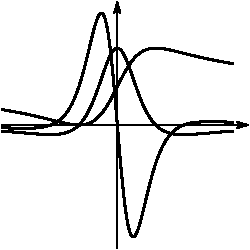
\includegraphics{08unlabeledgraphs.pdf}}
        \put( 74.75,  97.88){\sffamily\itshape \bf C}
    \put( 70.22,  69.47){\sffamily\itshape \bf B}
    \put( 71.22,  21.83){\sffamily\itshape \bf A}
\end{picture}

\end{center}

\problem \groupproblem Below is the graph of a function $y=f(x)$. %{{{3
\begin{center}
  
    \begin{picture} (120.000000,90.500000)(0,0)
    \put(0.0, 0.0){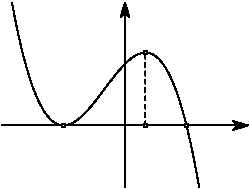
\includegraphics{08f-is-given.pdf}}
        \put(  7.90,  84.36){\sffamily\itshape $y=f(x)$}
    \put( 30.50,  20.50){\sffamily\itshape $a$}
    \put( 69.83,  20.50){\sffamily\itshape $b$}
    \put( 92.50,  32.50){\sffamily\itshape $c$}
\end{picture}

\end{center}
The function $F(x)$ (graph not shown) is an antiderivative of $f(x)$.
Which of the following statements are true?

\subprob $F(a)=F(c)$ 

\subprob $F(b)=0$ 

\subprob $F(b)>F(c)$ 

\subprob $F(x)$ has exactly 2 inflection points.

$ \spadesuit $

\begingroup\itshape
Use a substitution to evaluate the following integrals:
\endgroup



\problem  \(\DS \int_1^2\frac{u\, d u}{1+u^2}\) %{{{3

\problem \(\DS \int_0^5 \frac{x\, dx}{\sqrt{x+1}}\) %{{{3

\problem \(\DS \int_1^2 \frac{x^2\, dx}{\sqrt{2x+1}}\) %{{{3

\problem \(\DS \int_0^5 \frac{s\, ds}{\sqrt[3]{s+2}}\) %{{{3

\problem \(\DS \int_1^2\frac{x\, d x}{1+x^2}\) %{{{3

\problem \(\DS \int_0^\pi \cos\left(\theta+\dfrac{\pi}{3}\right)d\theta\) %{{{3

\problem \(\DS \int \sin\left(\frac{\pi+x}{5}\right) dx\) %{{{3

\problem \(\DS \int \frac{\sin 2x}{\sqrt{1+\cos 2x}} \,dx\) %{{{3

\problem \(\DS \int_{\pi/4}^{\pi/3} \sin^2\theta\cos\theta\, d \theta \) %{{{3

\problem \(\DS \int_{2}^{3} \frac{1}{r\ln r}\, dr\) %{{{3

\problem \(\DS \int \frac{\sin 2x}{1+\cos^2x}\,dx\) %{{{3

\problem \(\DS \int \frac{\sin 2x}{1+\sin x}\,dx \) %{{{3

\problem \(\DS \int_{0}^{1} z\sqrt{1-z^2}\, d z\) %{{{3

\problem \(\DS \int_1^2 \frac{\ln 2x}x \, d x\) %{{{3

\problem \(\DS \int_{0}^{\sqrt{2}} \xi (1+2\xi^2)^{10} \, d \xi \) %{{{3

\problem \(\DS \int_{2}^{3} \sin \rho \bigl(\cos 2\rho)^4 \, d\rho\) %{{{3

\problem \(\DS \int \alpha e^{-\alpha^2}\, d\alpha\) %{{{3

\problem \(\DS \int \frac{\DS e^{\frac1t}}{t^2}\, d t \) %{{{3

\end{multicols}
\noproblemfont

